\documentclass{standalone}

\usepackage[OT1]{fontenc}
\renewcommand*\familydefault{\sfdefault}
\usepackage{helvet,sfmath}
\usepackage{siunitx}

\usepackage{tikz}
\usetikzlibrary{arrows,calc,patterns}
% \usetikzlibrary{intersections, calc, arrows.meta}
\usepackage{tikz,tkz-euclide}

\begin{document}

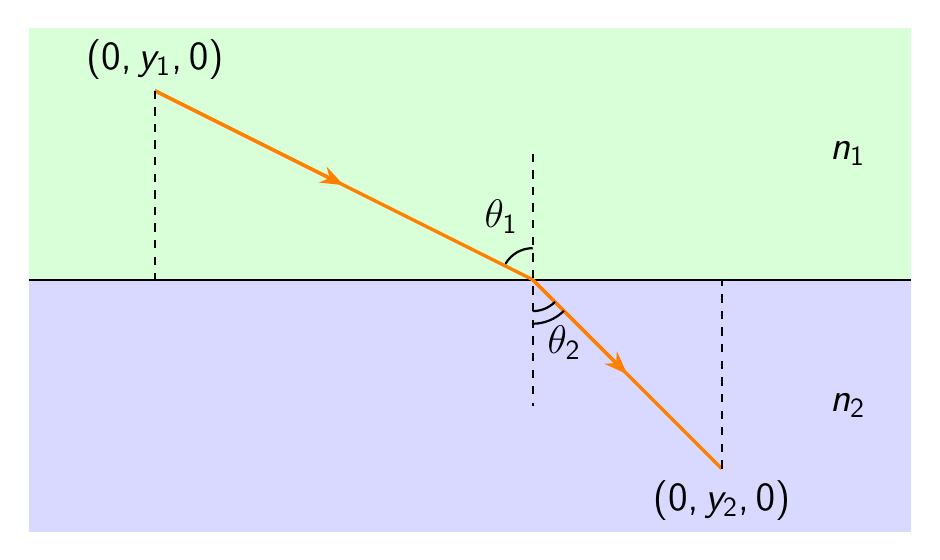
\begin{tikzpicture}[scale=0.8]
    %%Background
    \draw[draw=none, fill=blue!15] (-8,-4) rectangle (6,0);
    \draw[draw=none, fill=green!15] (-8,4) rectangle (6,0);
    \draw[thick] (-8,0) to (6,0);
    %% Light
    \draw[orange, very thick] (-6,3) to (0,0);
    \draw[orange, very thick] (0,0) to (3,-3);
    \draw[orange, very thick, -Stealth] (-6,3) to (-3,1.5);
    \draw[orange, very thick, -Stealth] (0,0) to (1.5,-1.5);

    \draw[dashed, thick]
    (-6,3) to (-6,0)
    (0,2) to (0,-2)
    (3,-3) to (3,0)
    ;
    \draw[thick]
    (0,0.5) arc (90:150:0.5)
    (0,-0.5) arc (270:315:0.5)
    (0,-0.7) arc (270:315:0.7)
    ;
    \draw
    (-6,3.5) node{\Large\(\left(0,y_1,0\right)\)}
    (3,-3.5) node{\Large\(\left(0,y_2,0\right)\)}
    (-0.5,1) node{\Large\(\theta_1\)}
    (0.5,-1) node{\Large\(\theta_2\)}
    (5,2) node{\Large\(n_1\)}
    (5,-2) node{\Large\(n_2\)}
    ;
\end{tikzpicture}

\end{document}
